\chapter{Appendix to Chapter 2}

\section{Ergodic and anisotropic distribution functions for dark-matter halos and their stellar halos in \texorpdfstring{\lowercase{\texttt{galpy}}}{galpy}}

\label{ch2:dfappendix}

To model the kinematics of the stellar halo and spherical galactic components more generally, we have implemented various spherical distribution functions in the \texttt{galpy} code. In this Appendix, we provide a brief overview of the implemented functionality and its mathematical basis that serves as a reference for the code. We consider distribution functions $f(E,L)$ embedded in a spherical potential $\Phi(r)$ that are functions of the specific energy $E$ and the total specific angular momentum $L$ and that have either constant orbital anisotropy $\beta$ or anisotropy of the Osipkov-Merritt type. Such models are standard textbook material \parencite[e.g.][]{binney08}, but for completeness we review the main theory behind them here.

\subsection{Spherical coordinates}

We work in spherical coordinates $(r,\phi,\theta)$, with $\theta$ the polar angle measured from the pole and $\phi$ the azimuthal angle. In terms of the usual cartesian coordinates $(x,y,z)$, the spherical coordinates are given by
\begin{align}
    \nonumber r       &= \sqrt{x^2 + y^2 + z^2}\,,\\
    \phi    &= \mathrm{atan2}(y,x)\,,\\
    \nonumber \theta  &= \pi/2 - \mathrm{atan}(z/\sqrt{x^2+y^2})\,,
\end{align}
and the inverse transformation is
\begin{align}
    \nonumber x  &= r\,\sin \theta\, \cos \phi\,,\\
    y  &= r\,\sin \theta\, \sin \phi\,,\label{ch2:eq-sphere-coords}\\
    \nonumber z  &= r\,\cos \theta\,.
\end{align}
In the spherical coordinate frame, the velocities  $(v_r,v_\phi,v_\theta)$ are given in terms of the cartesian velocities $(v_x,v_y,v_z)$ as
\begin{align}
    \nonumber v_r & = \phantom{-}v_x\,\sin\theta\,\cos\phi+v_y\,\sin\theta\,\sin\phi+v_z\,\cos\theta\\
    v_\phi & = -v_x\,\sin\phi\phantom{\,\cos\phi}+v_y\,\cos\phi\\
    \nonumber v_\theta & = \phantom{-}v_x\,\sin\theta\,\cos\phi+v_y\,\sin\theta\,\sin\phi-v_z\,\cos\theta\,,
\end{align}
with inverse transformation
\begin{align}
    \nonumber v_x & = v_r\,\sin\theta\,\cos\phi-v_\phi\,\sin \phi+v_\theta\,\cos\theta\,\cos\phi\\
    v_y & = v_r\,\sin\theta\,\sin\phi+v_\phi\,\cos\phi+v_\theta\,\cos\theta\,\sin \phi\label{ch2:eq-vel-spher}\\
    \nonumber v_z & = v_r\,\cos\theta\phantom{\,\sin\phi+v_\phi\,\cos\phi}-v_\theta\,\sin\theta\,.
\end{align}
When working with the velocities, we will also express them using a spherical coordinate system $(v,\psi,\eta)$ of their own, writing the velocities as
\begin{align}
    \nonumber v_{r} & = v \cos\eta\,, \\
     v_{\theta} & = v \sin \eta \cos \psi \label{ch2:eq-sphervels}\\
    \nonumber v_{\phi} & = v \sin \eta \sin \psi\,.
\end{align}
In these coordinates, the specific energy is
\begin{equation}\label{ch2:eq:E-as-v}
    E = \Phi(r) + {v^2 \over 2}\,,
\end{equation}
while the total specific angular momentum is given by
\begin{equation}
    L = rv\sin \eta\,,
\end{equation}
A distribution function $f(E,L)$ is therefore only a function of $(r,v,\eta)$ and does not depend on the two spatial angles $(\phi,\theta)$ or the velocity angle $\psi$.

The orbital anisotropy $\beta$ for our DFs is defined as
\begin{equation}
    \beta = 1-{\sigma_\theta^2+\sigma_\phi^2 \over 2\sigma_r^2} = 1-{\sigma_t^2 \over 2\sigma_r^2}\,,
\end{equation}
where $\sigma_{r,\phi,\theta}$ are the velocity dispersions in the radial, azimuthal, and polar directions and all quantities are measured at a given radius $r$; the second equality uses the velocity dispersion in the tangential velocity $v_t = v\,\sin\eta$.

\subsection{Distribution functions}

As is usual, we work in terms of the relative potential $\Psi = -\Phi+\Phi(\infty)$ and the specific binding energy $\mathcal{E} =  -E +\Phi(\infty) = \Psi -\frac{1}{2}\,v^2$. Bound orbits then have $0 < \mathcal{E} < \mathcal{E}_{\mathrm{max}}$, where $\mathcal{E}_{\mathrm{max}}$ is the maximum binding energy given by $\mathcal{E}_{\mathrm{max}} = \Psi(0) = -\Phi(0)+\Phi(\infty)$.

The first type of spherical DF that we consider are the \emph{ergodic DFs}
\begin{equation}
    f(\mathcal{E},L) \equiv f(\mathcal{E})\,.
\end{equation}
Because $\mathcal{E}$ does not depend on $\sin\eta$ (Equation \ref{ch2:eq:E-as-v}), such DFs have $\beta=0$ and are therefore isotropic. For a given density $\rho(r)$ embedded in a spherical potential $\Psi$, the DF is given by the Eddington inversion \parencite{eddington16}
\begin{equation}\label{ch2:eq-eddington-alt}
    f(\mathcal{E}) = \frac{1}{\sqrt{8}\,\pi^2}\,\frac{\mathrm{d}}{\mathrm{d}\mathcal{E}}\,\int_0^\mathcal{E}\mathrm{d}\Psi\,\frac{1}{\sqrt{\mathcal{E}-\Psi}}\,\frac{\mathrm{d}\rho}{\mathrm{d}\Psi}\,,
\end{equation}
or, equivalently,
\begin{equation}\label{ch2:eq-eddington}
    f(\mathcal{E}) = \frac{1}{\sqrt{8}\,\pi^2}\,\left[\int_0^\mathcal{E}\mathrm{d}\Psi\,\frac{1}{\sqrt{\mathcal{E}-\Psi}}\,\frac{\mathrm{d}^2\rho}{\mathrm{d}\Psi^2} +\frac{1}{\sqrt{\mathcal{E}}}\,\frac{\mathrm{d}\rho}{\mathrm{d}\Psi}\Bigg|_{\Psi=0}\right]\,.
\end{equation}
Note that the density $\rho(r)$ does not have to be related to the potential $\Psi$ through the Poisson equation; this is the case for the anisotropic DFs below as well. We will only deal with DFs where the last term is zero.

DFs with a constant, but non-zero, value of the anisotropy $\beta$ can be obtained using the form
\begin{equation}\label{ch2:eq-constantbetadf-form}
    f(\mathcal{E},L) \equiv L^{-2\beta}\,f_1(\mathcal{E})\,.
\end{equation}
As shown by \textcite{cuddeford91} \parencite[see also][for a clearer statement of this result]{an06}, for a given density $\rho(r)$ embedded in a spherical potential $\Psi$, the DF is given by the inversion 
\begin{equation}\label{ch2:eq-anidf-constbeta-generalsol}
\begin{split}
    f(\mathcal{E},L) =  & {2^\beta\,L^{-2\beta} \over (2\pi)^{3/2}\,\Gamma(1-\alpha)\,\Gamma(1-\beta)}\\&\ \times \left[\int_0^\mathcal{E}\mathrm{d}\Psi\,{1\over (\mathcal{E}-\Psi)^\alpha}\,{\mathrm{d}^{m+1} \over \mathrm{d} \Psi^{m+1}}\Big(\rho(\Psi)\,[r(\Psi)]^{2\beta}\Big)\right.\\& \quad \left. +{1\over \mathcal{E}^\alpha}\,{\mathrm{d}^{m} \over \mathrm{d} \Psi^{m}}\Big(\rho(\Psi)\,[r(\Psi)]^{2\beta}\Big)\Big|_{\Psi=0}\right]\,,
\end{split}
\end{equation}
where $m = \lfloor 3/2-\beta \rfloor$ and $\alpha = 3/2-\beta-m$. For half-integer values of $\beta$, the DF is simply given by
\begin{equation}\label{ch2:eq-anidf-constbeta-halfinteger}
    f(\mathcal{E},L) = {L^{-2\beta} \over 2\pi^2\,(-2\beta)!!}\,{\mathrm{d}^{3/2-\beta} \over \mathrm{d} \Psi^{3/2-\beta}}\Big(\rho(\Psi)\,[r(\Psi)]^{2\beta}\Big)\,,\quad 1/2-\beta \in \mathbb{N}\,.
\end{equation}
where $(-2\beta)!! = 2^{1/2-\beta}\,\Gamma(1-\beta)/\sqrt{\pi}$.

\begin{figure}
	\centering
	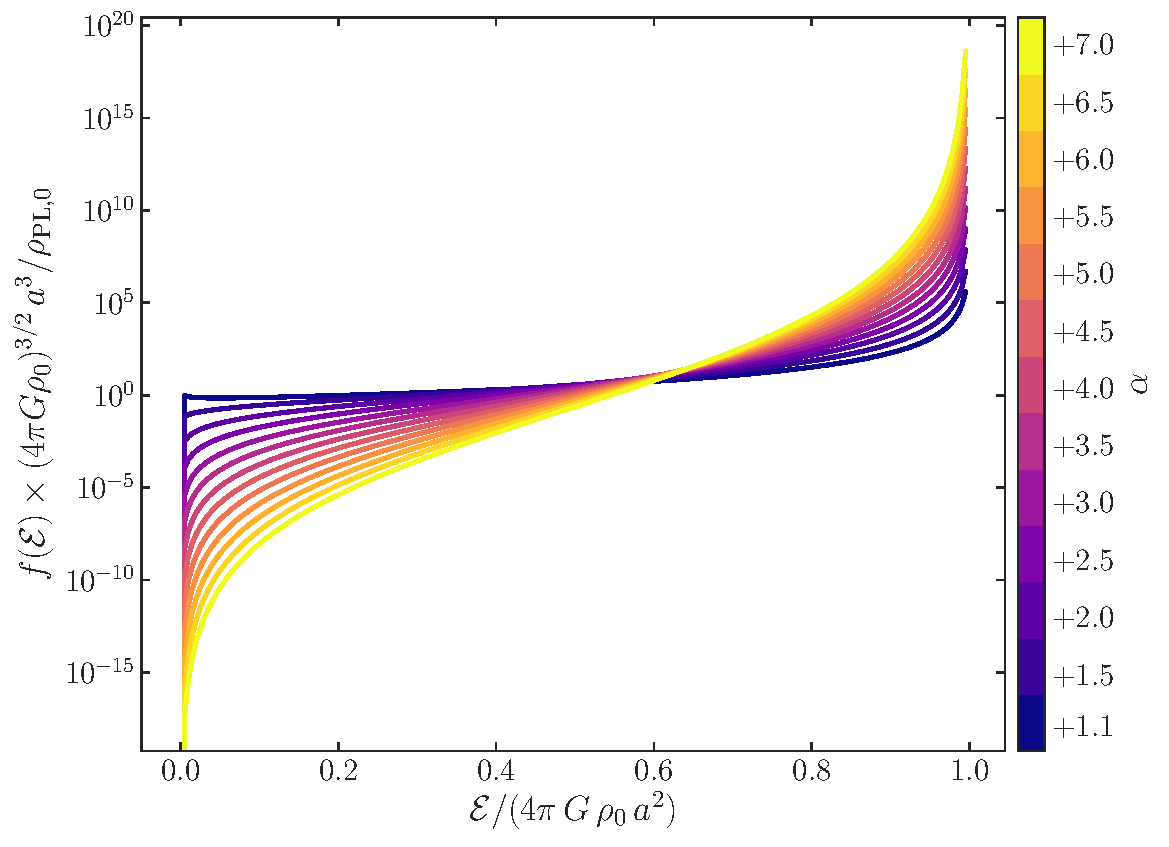
\includegraphics[width=0.75\textwidth]{figure/ch2/pl_in_nfw.pdf}
	\caption{Ergodic distribution function $f(\mathcal{E})$ for a power-law density profile $\rho(r) = \rho_{\mathrm{PL},0} (r/a)^{-\alpha}$ embedded in an NFW potential $\Phi(r) = -4\pi\,G\,\rho_0\,a^2\,\ln(1+r/a)/(r/a)$ in terms of the dimensionless binding energy $\mathcal{E}/(4\pi\,G\,\rho_0\,a^2)$.}
	\label{ch2:fig:pl_in_nfw}
\end{figure}

As first proposed by \textcite{osipkov79} and \textcite{merritt85}, DFs for a given density $\rho$ embedded in a gravitational potential $\Psi$ with radially-varying anisotropy of the form
\begin{equation}\label{ch2:eq-anidf-osipkov}
    \beta(r) = {1 \over 1+r_a^2/r^2}\,,
\end{equation}
can be obtained from DFs of the form
\begin{equation}
    f(\mathcal{E},L) \equiv f(Q)\,,
\end{equation}
where
\begin{equation}
    Q = \mathcal{E}-{L^2 \over 2r_a^2}\,,
\end{equation}
with $r_a$ the anisotropy radius (the radius where $\beta = 1/2$). For a given density $\rho$ embedded in a potential $\Psi$, this DF is given by an Eddington-like inversion
\begin{equation}
\begin{split}
    f(Q) =  \frac{1}{\sqrt{8}\,\pi^2}\,& \left[ \int_0^Q\mathrm{d}\Psi\,\frac{1}{\sqrt{Q-\Psi}}\,\frac{\mathrm{d}^2}{\mathrm{d}\Psi^2}\Big[\rho(\Psi)\,(1+r^2[\Psi]/r_a^2)\Big]\right.\\&  \ \left. +\frac{1}{\sqrt{Q}}\,\frac{\mathrm{d}}{\mathrm{d}\Psi}\Big[\rho(\Psi)\,(1+r^2[\Psi]/r_a^2)\Big]\Big|_{\Psi=0}\right]\,.
\end{split}
\end{equation}
This can also be written as
\begin{equation}\label{ch2:eq-spherdf-omdf}
\begin{split}
    f(Q) = f^{\beta=0}(Q)+\frac{1}{\sqrt{8}\,\pi^2\,r_a^2}\,&\left[\int_0^Q\mathrm{d}\Psi\,\frac{1}{\sqrt{Q-\Psi}}\,\frac{\mathrm{d}^2}{\mathrm{d}\Psi^2}\Big[\rho(\Psi)\,r^2(\Psi)\Big]\right.\\ & \ \left.+\frac{1}{\sqrt{Q}}\,\frac{\mathrm{d}}{\mathrm{d}\Psi}\Big[\rho(\Psi)\,r^2(\Psi)\Big]\Big|_{\Psi=0}\right]\,,
\end{split}
\end{equation}
where $f^{\beta=0}(Q)$ is the ergodic DF from Equation \eqref{ch2:eq-eddington} evaluated at $\mathcal{E} = Q$. Because the square brackets in the second term do not depend on $r_a$, Osipkov-Merritt DFs for a given $(\rho,\Psi)$ pair for all values of $r_a$ can be efficiently computed from two one-dimensional quadratures that do not depend on $r_a$.

\subsection{Numerical implementation}

\begin{figure}
	\centering
	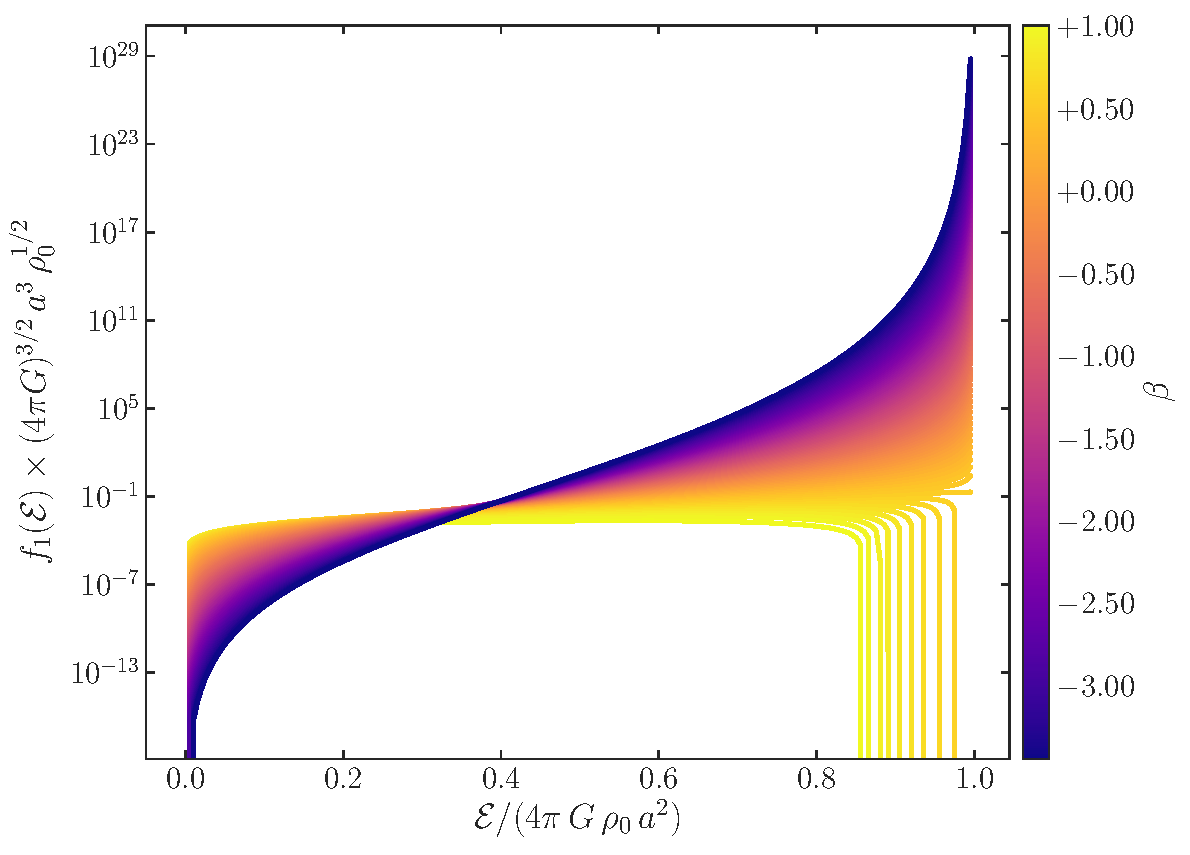
\includegraphics[width=0.75\textwidth]{figure/ch2/constantbeta_nfw.pdf}
	\caption{Energy part $f_1(\mathcal{E})$ of the self-consistent distribution function for an NFW profile with constant anisotropy $\beta$ for a dense grid in $\beta$. At $\beta > 0.5$, the distribution function becomes increasingly unphysical.}
	\label{ch2:fig:constantbeta_nfw}
\end{figure}

All of the DFs given in the previous subsection can be computed through one-dimensional quadratures over the relative potential $\Psi$. The only exception to this are the half-integer-$\beta$ constant-anisotropy DFs from Equation \eqref{ch2:eq-anidf-constbeta-halfinteger}, which do not require a numerical quadrature and are therefore straightforward to compute. The numerical integrals are difficult to compute for two reasons: (i) the integral is over $\Psi$, but the density is expressed as a function of $r$ and the integrand is therefore most easily evaluated as a function of $r$, and (ii) the integrand diverges integrably at the upper limit. To deal with difficulty (i), we rewrite all integrals to be over $r$ rather than $\Psi$; this requires the Jacobian $\mathrm{d} \Psi / \mathrm{d} r$, which is simply equal to the gravitational field. We also need to transform the limits of the integration: the lower limit of $\Psi = 0$ is the maximum radius $r_{\mathrm{max}}$ of the system and is typically infinity, the upper limit $\Psi = \mathcal{E}$ is transformed to $r$ by interpolating the function $r(\Psi)$. Because the integral after this transformation is well-behaved, the numerical error is easily dominated by how well this interpolation works and we therefore use a fine, logarithmically-spaced grid of $r$ values to determine $r(\Psi)$. After the transformation, the integral extends from $r(\mathcal{E})$ to $r=r_{\mathrm{max}}$ and when $r_{\mathrm{max}}=\infty$, this means that special handling of the integral is required at both limits: dealing with the integrable divergence at one end and an infinite limit at the other end. To deal with this, we split the integral at twice the lower limit and then use standard transformation methods to deal with the divergence and the infinite limit \parencite[e.g.][]{press07}. 

The implementation of the Eddington inversion in Equation \eqref{ch2:eq-eddington-alt} requires the second derivative of the density with respect to $\Psi$, while the constant-anisotropy DFs require derivatives of $\rho\,r^{2\beta}$ and the Osipkov-Merritt DFs need derivatives of $\rho\,r^{2}$. To compute these, we first of all rewrite them all as derivatives with respect to $r$ using the chain rule; this introduces derivatives of the relative potential that can be expressed in terms of the gravitational field and higher order derivatives of $\Psi$. For ergodic and Osipkov-Merritt DFs we only need at most two derivatives of either $\rho$ or $\Psi$ and to compute these, we explicitly add the first and second derivative of the density to all \texttt{galpy} spherical potentials; second derivatives of the potential already existed. Depending on how low $\beta$ goes, we need arbitrary derivatives of $\rho$ and $\Psi$ with respect to $r$. Rather than computing these by hand, we use \texttt{jax} \parencite{jaxgithub18}, a Python library that implements automatic differentiation of arbitrary functions built using \texttt{numpy} functions and more and that as such can compute arbitrary derivatives of functions to machine precision. To use \texttt{jax} in our case, we implement $\mathrm{d} (\rho\,r^{2\beta})/\mathrm{d} r$ as well as the radial field $\mathrm{d} \Psi / \mathrm{d}r$ using \texttt{jax}'s version of \texttt{numpy}. Note that for many potentials, the density derivative or the radial field does not involve special functions and it is then not actually necessary to load \texttt{jax}'s \texttt{numpy} implementation. The \texttt{jax} derivatives are also used to compute the necessary derivatives in the half-integer case of Equation \eqref{ch2:eq-anidf-constbeta-halfinteger}.

As an example of our numerical implementation, we display the ergodic DF $f(\mathcal{E})$ calculated using Equation \eqref{ch2:eq-eddington-alt} for a power-law density profile $\rho(r) = \rho_{\mathrm{PL},0} (r/a)^{-\alpha}$ that is embedded in an NFW potential with scale parameter $\alpha$
\begin{equation}\label{ch2:eq-nfw-pot}
\Phi(r) = -4\pi\,G\,\rho_0\,a^2\,\ln(1+r/a)/(r/a)\,
\end{equation}
in Figure \ref{ch2:fig:pl_in_nfw} for different values of the power-law exponent $\alpha$. As expected, more centrally-concentrated profiles with higher values of $\alpha$ have more stars on tightly-bound orbits. All of these DFs are physical, that is, do not contain negative regions.

A further example of our numerical implementation is given in Figure \ref{ch2:fig:constantbeta_nfw}, which shows the $f_1(\mathcal{E})$ part of the self-consistent DF for an NFW profile with constant anisotropy $\beta$ for a dense grid in $\beta$. The smoothness of the variation of the DF's shape with $\beta$ provides a good indication of the high numerical fidelity of our implementation. At $\beta > 0.5$, an increasingly large region at high binding energy is negative, indicating that there is no physical DF with such high constant anisotropy of the form of Equation \eqref{ch2:eq-constantbetadf-form}.

\subsection{Sampling the distribution functions}

To be able to sample six-dimensional phase-space coordinates for a wide range of spherical DFs, we have implemented exact random sampling for all of the DFs described in this Appendix. For all DFs, we sample positions $(r,\phi,\theta)$ by sampling $r$ from the cumulative mass profile, using inverse transform sampling, and sampling random angles on the sphere $(\theta,\phi)$ keeping in mind that while the distribution of $\phi$ is uniform on $ \phi \in [0,2\pi]$, the distribution of $\theta$ is $p(\theta)\propto \sin \theta$ on $\theta \in [0,\pi]$. Here and below, when the inverse cumulative distribution used in inverse transform sampling cannot be computed analytically, we calculate it using interpolating the inverse transform computed on a grid.

Sampling velocities necessarily depends on the anisotropy profile of the DF. For all DFs, we sample velocities in the spherical velocity coordinate system $(v,\psi,\eta)$ from Equation \eqref{ch2:eq-sphervels}. For DFs that only depend on $E$ and $L$, the distribution of the angle $\psi$ is uniform on $\psi \in [0,2\pi]$. For ergodic DFs, the distribution of $\eta$ is $p(\eta) \propto \sin \eta$, which can be sampled exactly using inverse-transform sampling using the fact that the cumulative DF can be inverted analytically. For DFs with constant $\beta$, we have that $p(\eta) \propto \sin^{1-2\beta}\eta$, which can also be sampled using inverse transform sampling (although while the cumulative DF can be expressed using special functions, it cannot be inverted analytically). We then sample the magnitude of the velocity from $p(v|r) \propto v^2 f(\mathcal{E})$ or $p(v|r) \propto v^2 f_1(\mathcal{E})$ for non-zero, constant $\beta$ using inverse transform sampling between zero and $v = v_{\mathrm{esc}}(r)$.

Exactly sampling Osipkov-Merritt-type DFs is slightly more difficult and has to our knowledge not been discussed before. We first sample the velocity angle $\eta$ from $p(\eta|r) \propto \sin\eta\,[1+(r/r_a)^2 \sin^2\eta]^{-3/2}$ using inverse transform sampling. We then proceed to sample $v'=v\sqrt{1+(r/r_a)^2\sin^2 \eta}$ from $p(v'|r)\propto v'^2 f(Q)$. Remarkably, the cumulative distribution of $\cos \eta$ can be analytically inverted, so sampling it using inverse transform sampling is straightforward.

In practice, we interpolate the inverse cumulative distributions for $v$ or $v'$ in both the quantile and $r$ using two-dimensional interpolation. After this and other interpolations are set up, sampling the DFs is fast, achieving rates of $\approx 10^6$ points per second.

\subsection{Special cases and new ergodic and Osipkov-Merritt NFW distribution functions}

\begin{figure}
	\centering
	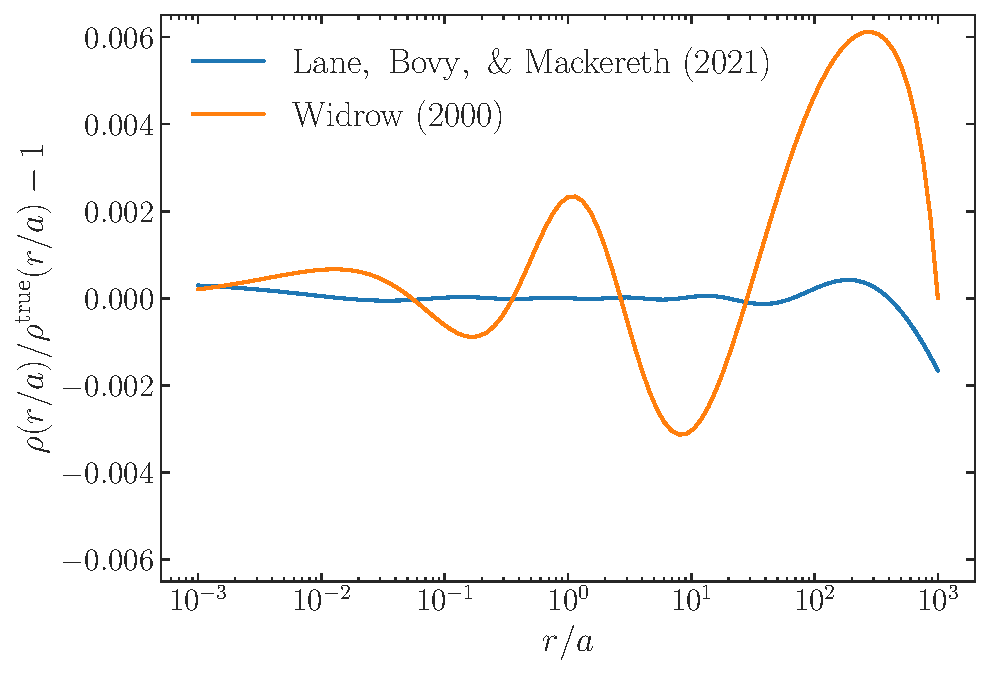
\includegraphics[width=0.6\textwidth]{figure/ch2/ergodic_nfw_denscomp.pdf}\\
	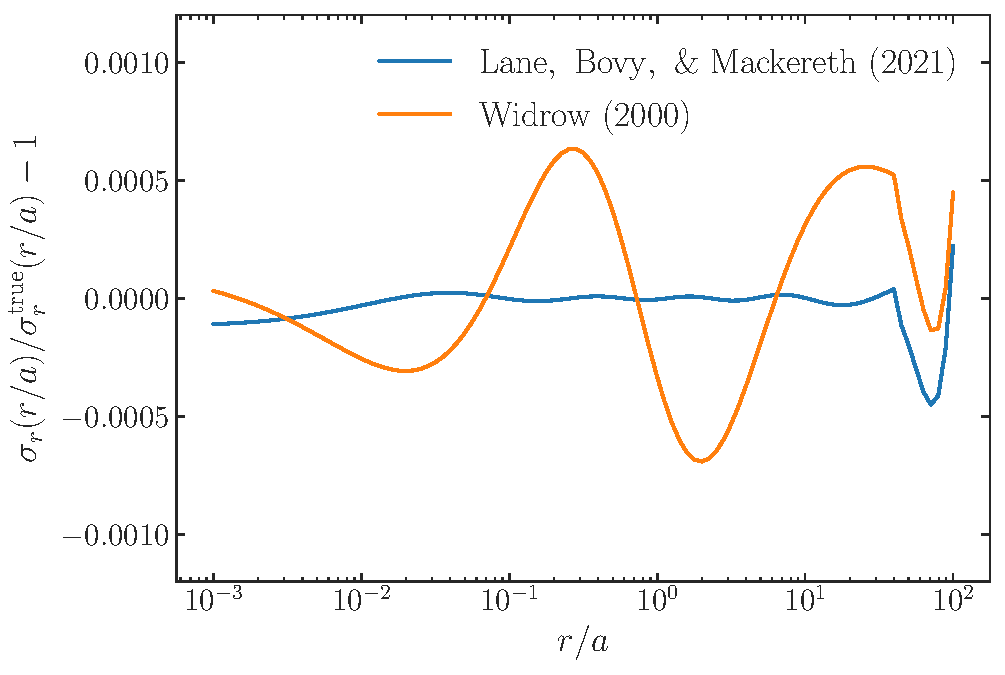
\includegraphics[width=0.6\textwidth]{figure/ch2/ergodic_nfw_sigmacomp.pdf}
	\caption{Recovery of the density and radial velocity dispersion of an NFW profile from the new form of Equation \eqref{ch2:eq-nfw-ergodic-newform} for its self-consistent distribution function. Compared to the simpler approximation from \textcite{widrow00}, the match to the density and velocity dispersion is better by more than an order of magnitude almost everywhere using our improved fitting function.}
	\label{ch2:fig:ergodic_nfw}
\end{figure}

Many analytic solutions for ergodic and anisotropic spherical DFs exist. Of these we have currently implemented:
\begin{itemize}
    \item The ergodic DF of a Hernquist profile \parencite{hernquist90};
    \item The Osipkov-Merritt-type DF of a Hernquist profile \parencite{hernquist90};
    \item The constant $\beta$ DF for a Hernquist profile for arbitrary $\beta$ \parencite{baes02};
    \item The ergodic DF of a Plummer profile $f(\mathcal{E}) \propto \mathcal{E}^{-7/2}$ \parencite[e.g.,][]{binney08};
    \item The \textcite{king66} DF \parencite[e.g.][]{michie63}.
\end{itemize}

Because NFW profiles describe the spatial distribution of simulated dark-matter halos well, self-consistent NFW DFs are of special interest. However, there is no known analytic form for the ergodic or general anisotropic DFs \parencite[however, see][for a notable exception, the DF with constant $\beta=1/2$]{evans06}. Approximate ergodic and Osipkov-Merritt-type DFs for the NFW profile were presented by \textcite{widrow00}. Using the high-fidelity numerical calculation obtained using our code of the ergodic and Osipkov-Merritt-type NFW DFs, we have found more complex, but more accurate fitting functions for these two cases. For the ergodic DF, we find that
\begin{equation}
\begin{split}\label{ch2:eq-nfw-ergodic-newform}
    f(\mathcal{E})\times&(4\pi G)^{3/2}\,a^3\,\rho_0^{1/2} \\&\!\!\!= \mathcal{E}^{3/2} \,(1-\mathcal{E})^{-5/2}\left({-\ln \mathcal{E} \over 1-\mathcal{E}}\right)^{-2.75}\\& \times \left(7.84806318891231\, \mathcal{E}^{10} - 41.0268009529576\, \mathcal{E}^{9}\right.\\& \quad\ + 92.5144063082258\, \mathcal{E}^{8} - 117.647787290798\, \mathcal{E}^{7}\\&\quad\ + 92.6397009471828\, \mathcal{E}^{6} - 46.6587221550258\, \mathcal{E}^{5}\\&\quad\ + 14.9776586391246\, \mathcal{E}^{4} - 2.97848277491979\, \mathcal{E}^{3}\\&\quad\ + 0.258346829924101\, \mathcal{E}^{2} + 0.0232272797489981\, \mathcal{E}\\&\left. \quad\ + 0.0926081086527954\right),
\end{split}
\end{equation}
where $\mathcal{E}$ is evaluated in its dimensionless form $\mathcal{E}/(4\pi\,G\,\rho_0\,a^2)$.
Figure \ref{ch2:fig:ergodic_nfw} compares the resulting density and radial-velocity dispersion profiles to their exact values, illustrating that this corresponds to the NFW profile better than the \textcite{widrow00} approximation.

For the Osipkov-Merritt-type DF for the NFW profile, we find that 
\begin{equation}
\begin{split}
    \huge[f(Q)&-f^{\beta=0}(Q)\huge]\times(4\pi G)^{3/2}\,a^3\,\rho_0^{1/2} \\&\!\!\!=  \left({a \over r_a}\right)^2\, {1 \over Q^{2/3}}\,\left({1-Q \over \ln Q}\right)^2\,\\
    & \times \left(- 0.995895790138335 \,Q^{8} + 4.29052661245253 \,Q^{7}\right.\\&\quad\
    - 7.60690467091859\, Q^{6} + 7.03132348658788\, Q^{5}\\&\quad\ - 3.6920719890718\, Q^{4} + 0.831302363461598\, Q^{3}\\&\quad\ - 0.217968733177408\, Q^{2} - 0.0408426627412238\, Q\\&\quad\ \left.+ 0.0802975743915827\right),
\end{split}
\end{equation}
where $Q$ is evaluated in its dimensionless form $Q/(4\pi\,G\,\rho_0\,a^2)$ and $f^{\beta=0}(Q)$ is the ergodic DF from Equation \eqref{ch2:eq-nfw-ergodic-newform} evaluated at $\mathcal{E} = Q$. Unlike the forms given by \textcite{widrow00}, our new form allows for an arbitrary value of $a/r_a$. How well the approximate DF recovers the density and radial velocity dispersion profile depends on $a/r_a$, but the density is typically recovered to within a few percent out to $100a$ and the velocity dispersion to better than one percent.
